\documentclass{book}

%\usepackage{w-bookps}

%%%%%%%%%%%%%%%%%%%%%%%%%%%%%%%%%%%%%%%%%%%%%%%%%%%%%%%%%%%%%%%%
%% Graphicx.sty for Including PostScript .eps files

\usepackage{graphicx}
\usepackage[cmex10]{amsmath}
\usepackage{amssymb}
\usepackage{epstopdf}
\usepackage{xfrac}
\usepackage{float}
\usepackage{psfrag}
%\usepackage{circuitikz}
%Enables Latex Example enviroment
\usepackage{showexpl}
%Circuit drawing packages
\usepackage[siunitx]{circuitikz}
\sisetup{load=derived} % loading \siemens

%Ploting packages
\usepackage{tikz}
\usepackage{pgfplots}


\usepackage{framed}

%Bibliography per chapter
\usepackage[square,numbers]{natbib}
%\usepackage{chapterbib}

\begin{document}

\title{Towards SC-enabled high density highly miniaturized power LED drivers: A model-centric optimization framework}


\author{J. Delos Ayllón \\
}


\maketitle

\pagenumbering{roman}
\tableofcontents
\listoffigures
\listoftables


%%%%%%%%%%%%%%%%%%%%%%%%%%%%%%%%
% \begin{introduction}
%\introauthor{<name>}{<affil>}
% Introduction text...
% \end{introduction}


%\begin{abstract}
%\end{abstract}

\pagenumbering{arabic}

\part{Towards Highly Miniaturized LED Power Systems }
\label{ch:twrd_HMLED}

\chapter{The new coming LED based lighting industry}

The appearance of light in the beginnings of the 19th century and the posterior commercialization was clearly a remarkable fact of the past history. The light bulbs contributed in two major facts that impacted peoples life . First, they enabled to have clear, reliable and safe source of light at home, extending our activity hours longer than the natural sun light. As a matter of fact we can not live without the use of artificial light.   Second, the necessity of electric power helped to develop the first electric power distribution systems. Actually, that fact can be still evidenced since people, generally our grand parents, often use the word \emph{light} when they actually are refereing electricity.

\begin{figure}[!h]
\centering
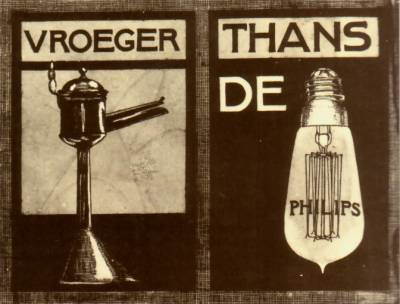
\includegraphics{./0_intro/img/1900-philips3.jpg}
\label{fig:incandescent_light_blub}
\caption{Early incandescent light bulb}
\end{figure}


From the first incandescent light bulb, the lighting industry has not had any big disruptive change to our perception of lighting till the last decade with the apparition of the LED lamps. Besides as many of us thing, it has been done a large effort to improve the efficiency of the light sources while keeping a the quality of the light as good as the incandescent light bulb. Being the florescent lamps one of the biggest contributions during the past century, beginning  to be commercialized around 1930. Later becoming a disruptive change in the lighting market with the introduction the low consumption lamps where Philips was one of the first player launching to the market the first screw-in fluorescent lamp. Although the prices of these lamps has been dropping to become commercially attractive for the costumers, their poorer color rendering factor and the longer setting time compared to the incandescent lamps prevented this lamps to be one-to-one replacement. Therefore the lighting industry has been keep without not too much attention till the introduction the LED based lamps.

\vspace{5mm} %5mm vertical space

\begin{figure}[!h]
\centering
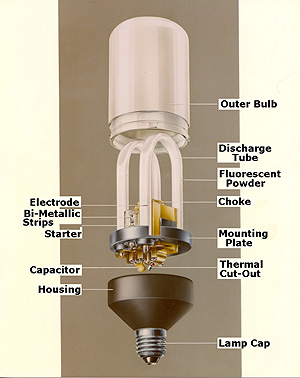
\includegraphics{./0_intro/img/phil1b.jpg}
\label{fig:philips_sl}
\caption{Components of the Philips SL compact fluorescent lamp. }
\end{figure}

The discovery of the high-efficiency blue LED ~\cite{94Nakamura} by Shuji Nakamura in 1994 enabled the quick development of the fist efficient withe LED. These early high power LEDs demonstrated that Solid State Lighting (SSL) devices  where a suitable technology for illumination. The relevance of Nakamura's work has been recognized last year being him awarded with the 2014 Nobel prize in physics. Looking farther we can also confirm the relevance of his invention since the apparition of the LED lamps, lighting is impacting again in our everyday life by changing our traditional concept of luminaries and lighting possibilities.

\begin{figure}[!h]
\centering
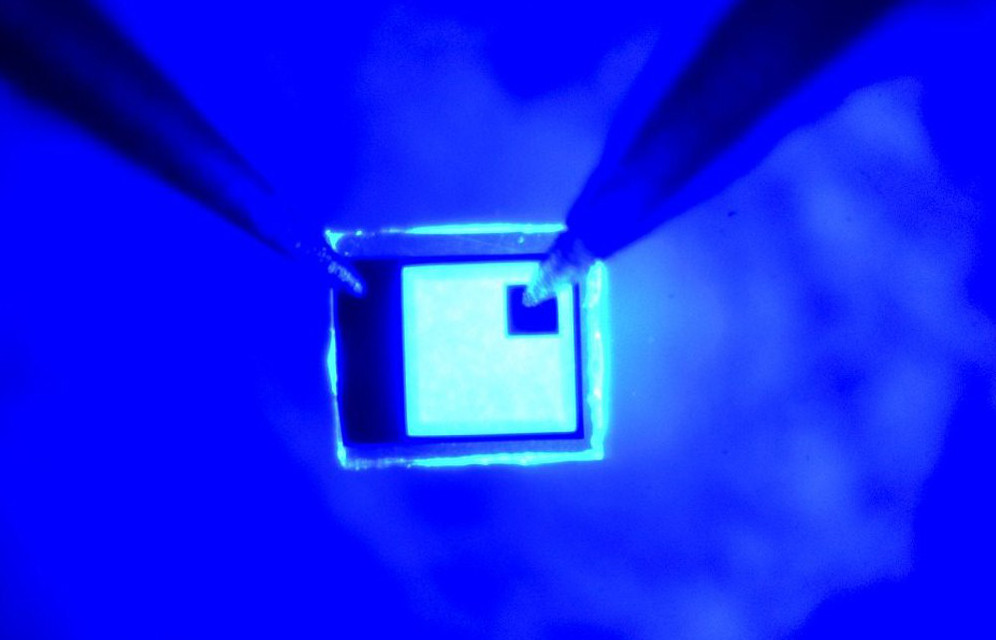
\includegraphics{./0_intro/img/10-7-14-nobel-prize-blue-led.jpg}
\label{fig:blue_LED}
\caption{Picture of a blue LED researched by Shuij Nakamura.}
\caption*{Source: \url{http://www.newsweek.com/how-blue-led-changed-world-and-won-nobel-prize-275977} }
\end{figure}

LED based lamps triggered  a frenetic rush in the lighting industry to bring that technology to the end consumers. Actually the large number of advantages of LED based lighting, or also known as Solid State Lighting (SSL), are so relevant that in the close future will replace any of the present lighting technology, that movement has been already named as the \emph{LEDification}. The principal advantages of SSL are:
\begin{description}
  \item [Efficiency] The light generation inside an LED is produced by the direct mechanism of hold-electron recombination, the supplied energy is a better use of the energy compared to the incandescent lamps. The power consumption can be up to an order of magnitude lower of an incandescent light.

  \item [Size] LEDs are tiny and flat devices, which can be considered as 2-D elements and do not need any vacuum chamber to work. They are much more flexible devices to assembly, and can easily replace the old glass made bulb design.

  \item [Color] LED light has a very narrow light spectrum, that can be used to produce directly colored light. Colored lights are becoming more popular in domestic homes becoming a piece of decoration or mood tweaking device.

  \item [Dynamics] Compared to any of the traditional sources of light LEDs have no dynamics, actually they have but it's very fast and not appreciable to the human eye. Therefore they do not have any setting time when turned on, which is not the case of CFL. The fast dynamics allows to modulate the light and transmit data without disturbing the human beings.

  \item [Lifetime] Solid State devices do not wear off, there fore they can be considered to have an infinite lifetime. In practice LEDs make use of organic phosphores, thus the light quality derates with the use, but the life expectancy of the LED is rated from 20.000 - 100.000 hours, multiplying 20 to 100 times longer that the classical light bulbs.
\end{description}

\vspace{5mm} %5mm vertical space

Bring the LED based lamps to the market is still a big challenge. Despite of the large number of advantages, the end consumers are still very reluctant to change generally due to the elevated costs of the new lamps, currently ranging between \$20 - \$40 for a 100W substitute compared to less than \$3 of an incandescent light. Also another issue that prevents consumers to change to the new technology is a poor light color consistency, light flickering and light dimming incompatibilities, that become really evident in low budget products.

\begin{figure}[!h]
\centering
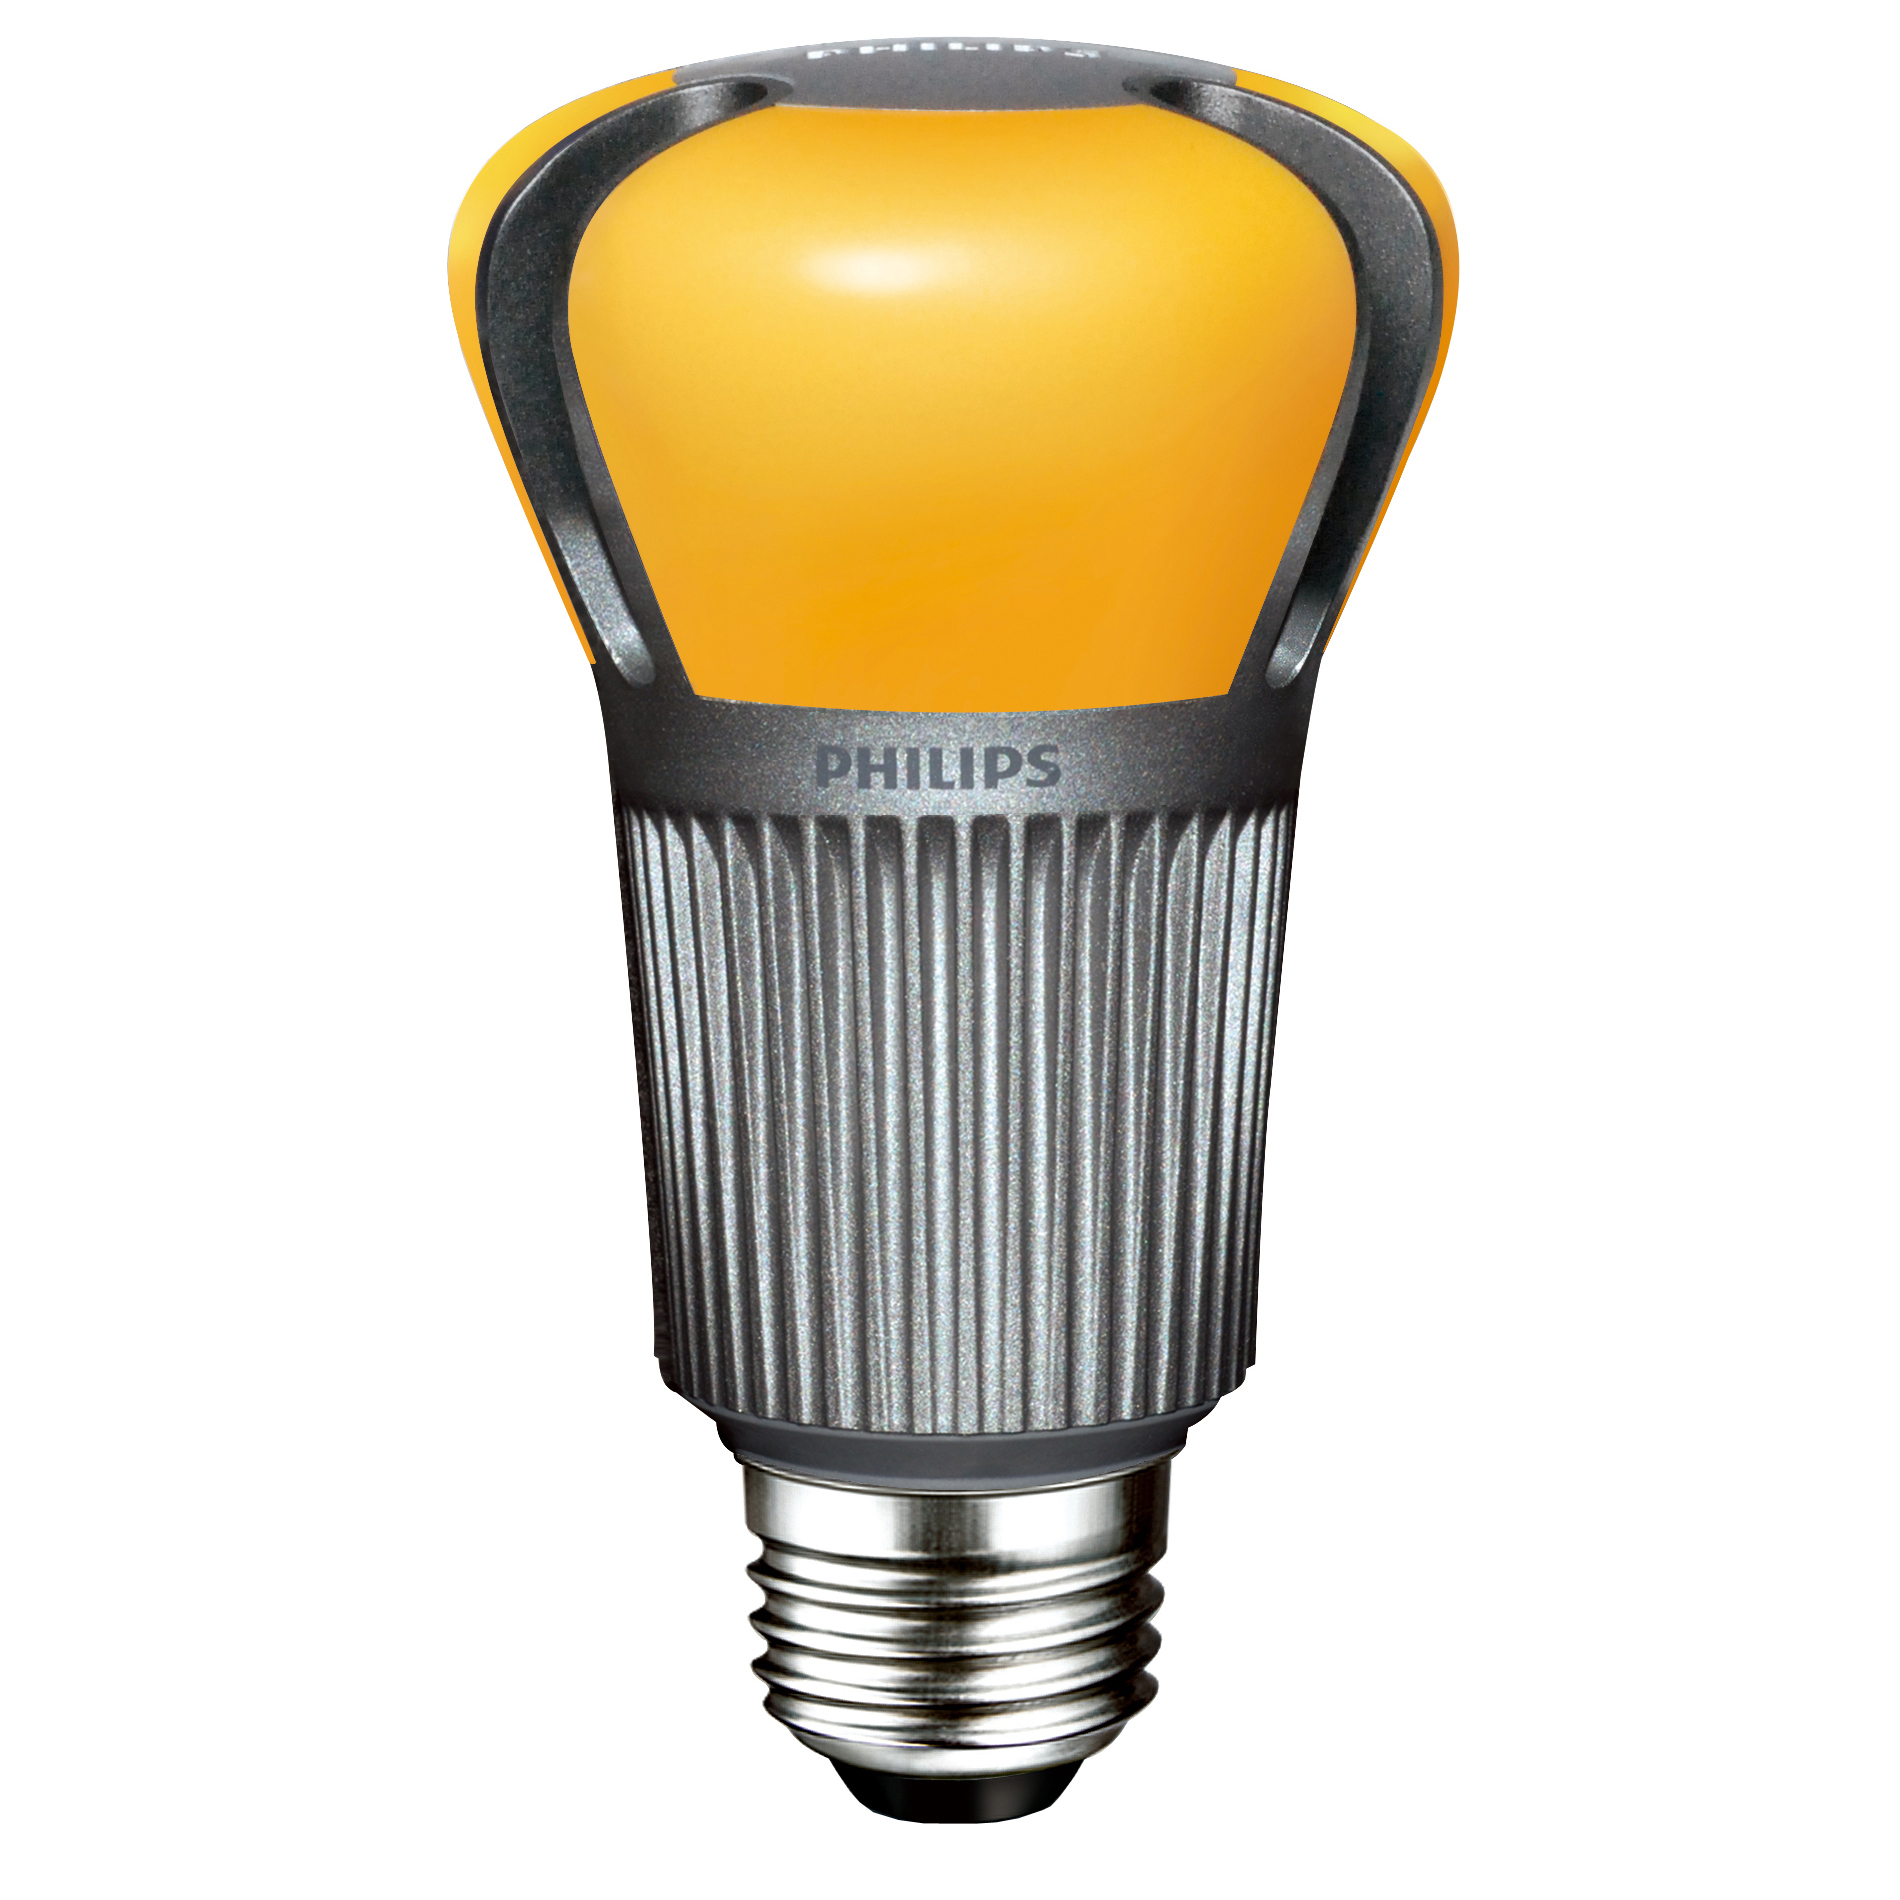
\includegraphics[width=4cm]{./0_intro/img/enduraled-12w.jpg}
\label{fig:l_prize}
\caption{900 lumens LED light bulb.}
\end{figure}

Two factors can be identified to make more favorable the adoption of the SSL as the preferred lighting solution by the consumers. In the one hand, reducing the end product price; and in the other hand, bringing more value to the traditional light sources. Actually LED light bulbs already bring more value compared to the old light bulbs being much more efficient, almost one order of magnitude lower in power consumption, and a longer lifetime, easily twenty times more operating hours. However these factors are not yet a valuable argument for the consumers. With the current trend of the \emph{internet-of-things} remote control, color tuning, light level dimming and integration to with future smart houses are probably some value propositions that people will need and SSL can easily provide. In a second level, I assume that the luminaries designs will change with a more favorable designs that take advantage of the low profiles of the LEDs.

 \begin{figure}[!h]
\centering
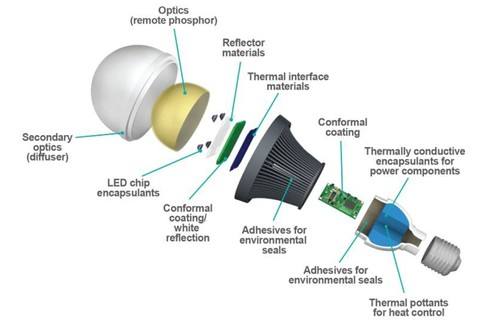
\includegraphics[width=8cm]{./0_intro/img/exploded_bulb_2.jpg}
\caption{Exploded vision of an LED light bulb.}
\label{fig:exploded_bulb}
\end{figure}

It is essential to describe the different elements in a LED light bulb in order to understand the challenges in its development and  design. A LED light bulb is composed by the six main elements described below and shown in  the Fig. ~\ref{fig:exploded_bulb}.

\begin{description}
  \item[LED] A two-lead semiconductor device that produced light when a current flows through it. The name comes from its acronym \emph{Light-Emitting Diode}. The light is produced by electroluminescence when an electron recombines with an electron-hole releasing energy in form of photons. The color of the light is determined by the energy band gap of the semiconductor.

   LED cost is very cheap and there is a broad assortment in colors, power and applications. The selection of the LED will determine: light color, voltage and current of the load, efficiency and necessary optics.

  \item[Optics] The optical device that helps to collimate, mix and distribute the light in the space in a desired way, normally uniformly for a determined projection area.

  \item[Driver] Electronic circuit placed between the input source and the load, the LEDs, that transforms the input electrical power to the requirements of the load. Since almost all the power distribution systems and storage devices are voltage sources and LEDs are current supplied loads, an LED driver is considered as current-to-voltage (V-I) power supply.

      The driver controls the current thought the load, hence the light output. Therefore it can be considered as the active part of the system where the control of the lamp relies. It is the most expensive and takes the largest volume of the lamp, and also one of the most or even the most important element in the entire system.

  \item[Heat sink] Mechanical element that acts as a passive heat exchanger and cools hot elements within the lamps system by dissipating the heat into the surrounding medium. The energy that is not converted to light becomes heat and must be extracted from the lamp, the main heat contributors elements are the LEDs and some components of the driver.

      The costs of the heat sink is also a relevant part in the total cost of the lamp.

  \item[Body assembly] Mechanical element that hold all the different subsystems in one single device. In many cases the heat sink does this functionality.

  \item[Connector] Mechanical element that provides connection with the energy source. The most popular one is the Edison connector present in all screw-in lamps. There are many other popular ones such as GU10, MR16, MR11 coming from the halogen multifaceted reflector bulbs or the 2-pin connector of the fluorescent tubes.

      In many cases, the standardized connectors suppose a restriction for the mechanical design of the lamp. Their old-fashioned design is not optimal for the new lamps.


\end{description}

\vspace{5mm} %5mm vertical space

The chart shown in Fig.\ref{fig:cost_breakdown} makes evident that the driver is the most expensive part of the system. As it was previously mentioned, the driver is the key component in the functionality of the LED lamp, since it controls the light output and at the same time determines the efficiency of the system. Therefore, the LED driver has become on of the hot topics of research within the power electronics field. Besides the necessity of fulfilling the operational requirements, such as high efficacy an proper power quality, two main issues have trigger research around the driver circuit: The costs and the volume.
\begin{figure}[!h]
\centering
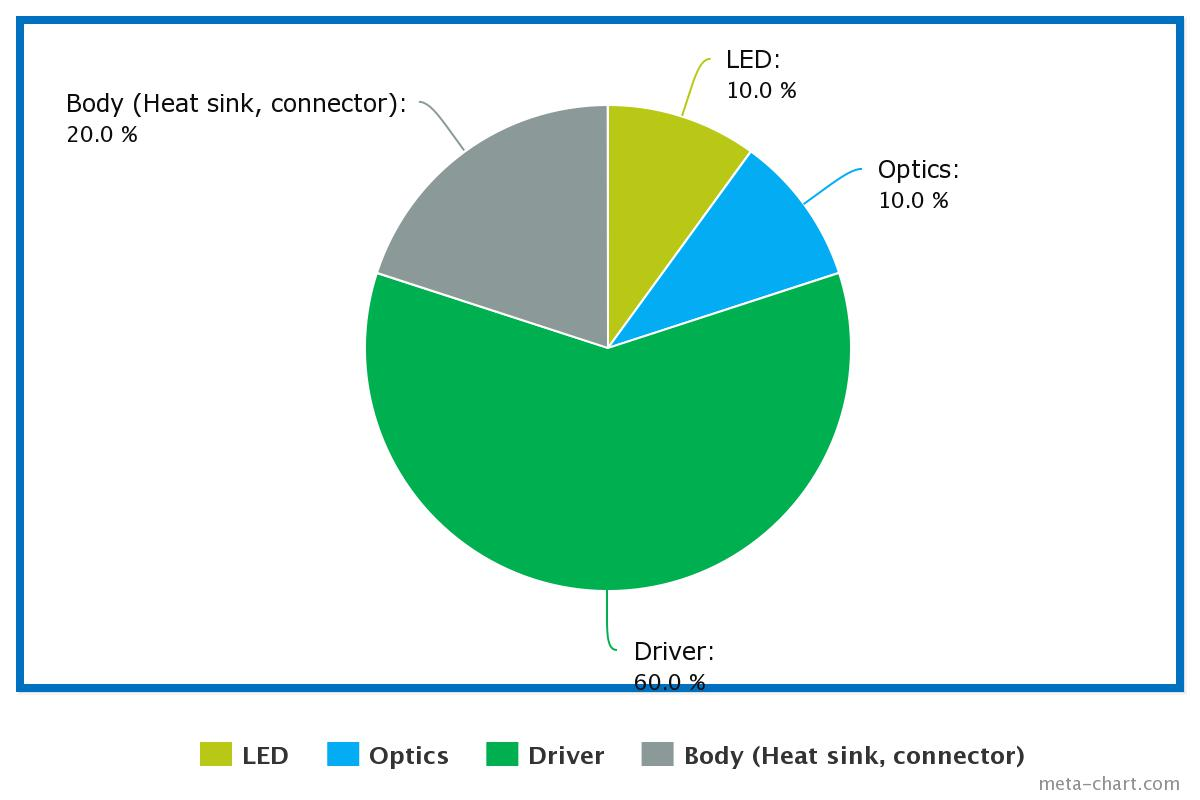
\includegraphics[width=8cm]{./0_intro/img/piechar_costs.jpeg}
\caption{LED lamp cost breakdown by subsystems.}
\label{fig:cost_breakdown}
\end{figure}

\vspace{5mm} %5mm vertical space

The cost of the driver is one of the biggest problems that SSL industry has been dealing after the power LEDs become a commodity components. Actually, this piece of electronics was not present in the incandescent light bulbs, thus its elevated cost arose as an inconvenient and difficult to justify in the new light bulbs. Philips Research has devoted a large effort in that field, being indeed the main focus of research regarding the LED drivers.


Reducing the costs of the lamps has been the strategy taken for the first wave in the \emph{LEDification} process where retrofitting\footnote{Adding the new LED technology to the older light bulb systems. In that way the end user can directly replace an incandescent lamp or a florescent tub by an LED one without needing to make any change in the current installation.} the old lamps is chosen as the way to target the end costumer. In on the one hand, fruitful results came form that research with new innovative solutions at very low costs that could be packed in almost all the light bulb shapes currently commercially available. But in the other hand, these new drivers had the incontinent of using very old components that at the same time restricted reduction of the circuit volume and made more complex the addition of extra control functionalities while keeping the initial low costs.

\begin{figure}[!h]
\centering
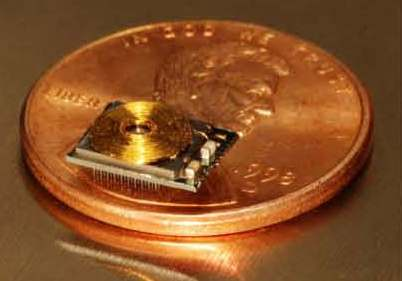
\includegraphics[width=8cm]{./0_intro/img/FSolzbacher01.jpg}
\caption{Power System in a Package die. The circuit implements a buck converter.}
\label{fig:psoc_example}
\end{figure}

\vspace{5mm} %5mm vertical space

The second line of research has focus on reducing the volume of the driver circuit. That research topic arose when comparing the the volume of the LEDs and the driver, it is evidenced a mismatch between the two volume of the components, becoming in many cases the driver circuit the dominant element of the entire lamp. Such mechanical constrain supposes an obstacle to take the full advantage of the low form-facto of the LED in the future luminaries, where LED will not be assembled using the old fashioned cases. Therefore, that research has a much longer term vision for targeting the second of third generation of lights in the \emph{LEDification} process.

The drive to reduce the volume of the drivers led to focus the research from the perspective of the integrated power supplies, where the power converter can be partially or fully integrated in a single package. There are two approaches of integrated power converters: \emph{Power System on Chip} (PSoC) or  \emph{Power System in Package} (PSiP). The first integrate all required power components, active and passive, in a single die. The second assemble all the components within the same package, keeping the appearance of an unique \emph{Integrated Circuit} (IC), see Fig.\ref{fig:psoc_example}. The advantages of having an integrated power management unit align with the necessities of the LED drivers, therefore trend of the drivers will be going towards having \emph{Power LED Drivers in Package} (PLDiP).

Besides the size reduction that an integrated driver would suppose, an integrated approach would also bring other benefits in terms of control and connectivity. Since such a solution would require a the design of a dedicated \emph{application-specific integrated circuit} (ASIC), the power management unit and driver control unit can be integrated together, providing the necessary intelligence for light control and the connectivity optimized for the requirements of the coming connected lighting industry. The \emph{Philips} \emph{HUE} lamp is a clear example of the requirements of the so called \emph{smart drivers}. That lamp provides a full light color gamut color control through a mobile and web application or through a remote control. The internal driver has four light channels red, green, orange and additional amber and at the same time provides wireless connectivity through ZigBee, being the electronic board populated with discrete power drivers and few micro-controller units. A solution that integrates all the functions in a single IC, or few ICs (one per channel), will definitely reduce packaging and assembling costs and still providing the same functionalities. And at the same time, the expected market size for LED lighting to justify a dedicated ASIC design for the light bulbs and indeed has been the motivation of this thesis. Therefore goal of this work was to explore and identify new architectures that are suitable for integration and at the same time can perform as an efficient LED driver.


\section{Why a LED needs a driver?}

As shown in Fig. \ref{fig:led_I-V} a LED has a very abrupt V-I curve. For voltages below the \emph{forward voltage}, $V_{f}$, there is no current flow and the LED behaves as an open circuit. For voltages above $V_{f}$ the curve becomes very steep and the current increases dramatically with respect to the voltages, thus the LED behaves as short circuit. The driver bias the LED to a specific point, $P$ in Fig. \ref{fig:led_I-V}, providing the desired output light. The colour and flux (light intensity) will vary depending of the bias point.  Since the majority of  available  energy sources are  voltage sources, and LED requires a circuit that limits the current that flows through it, that circuit is the LED driver.

\begin{figure}[!h]
\centering
\begin{tikzpicture}[domain=0:5]
    \draw [->] (0,0) -- (4.5,0) node[anchor=west]{$V$};
    \draw [->] (0,0) -- (0,4.5) node[anchor=east]{$I$};

    %Mark Vth
    \draw (2,2pt) -- (2,-5pt) node[anchor=north] {$V_{f}$};

    %Draw ideal plot
    \draw[thick] (0,0) -- (2,0) -- (4,4);

    %Draw bias points
    \draw[dashed] (3,2) -- (3,-0);
    \draw (3,2pt) -- (3,-5pt) node[anchor=north]  {$V_{bias}$};

    \draw[dashed] (3,2) -- (-0,2);
    \draw (2pt,2) -- (-5pt,2) node[anchor=east]  {$I_{bias}$};
    \filldraw (3,2) circle(2pt) node[anchor=west] {$P$};

  

\end{tikzpicture}
\caption {}
\label{fig:led_I-V}
\end{figure}

At the first glance, keeping a constant bias current, $I_bias$, through the LED does not seems to be challenging. However LED V-I characteristic is not static, in practice LEDs has different source of deviations and drivers have to deal with them in order to keep delivering the desired light output. First, $V_f$ has a negative dependence with the temperature, drooping its values as the PN junction temperature increases. Second, the LED has an aging factor derating its light output over time, which has to be adjusted by changing the bias point. And last but not least, during production LEDs will vary in colour, flux and forward voltage; even for products from the same batch. The manufacturer reduced the dispersion between devices by binning \footnote{Quality control performed at LED production line, where each LED is individual tested and sorted in groups (bins) that have the same electrical and lighting characteristics.}, but still after binning it can be deviations from up to $10\%$ in $V_f$ for the same part number.

Up to date, there are three families of LED drivers:

\begin{description}
  \item[Linear Drivers] place a shunt element between the source and the LED. The shunt element limits the current in the LED providing the necessary voltage droop between the source and the load. The excess of voltage between the source and the load is dissipated in the shunt element, literally burned in form of heat; therefore this drivers become very inefficient if the LED voltage is not close to the source. Moreover this drivers can only provide step-down conversion, thus they cannot work when the load voltage is higher than the input supply.

      \begin{figure}[!h]
        \centering
        \ctikzset { bipoles/length=1cm}
        \begin{circuitikz} [american,scale=0.65]
        \draw
        (5,0) to[short]
        (0,0) to[V = $v_{src}$]
        (0,3) to[generic=${Shunt}$]
        (5,3);
        \draw
        (5,0) to[leD*,mirror,v>=$v_{o}$,i<=$i_o$] (5,3); 
        
        \begin{scope}[xshift = 8cm, yshift=0cm]
            \draw[->] (0,0) -- (4,0) node[anchor=north] {$  m $};
            \draw[->] (0,0) -- (0,3) node[anchor=west] {$\eta $};
            
            %Ticks X 
            \draw (3,2pt) -- (3,-5pt) node[anchor=north] {$1$};
            \draw (1.5,2pt) -- (1.5,-5pt) node[anchor=north] {$0.7$};
            
            %Ticks Y
            \draw (2pt,2.5) -- (-5pt,2.5) node[anchor=east] {$100\%$};
            \draw (2pt,1.5) -- (-5pt,1.5) node[anchor=east] {$70\%$};
            
            %Markers
            \draw[dotted] (3,2.5) -- (3,0);
            \draw[dotted] (3,2.5) -- (0,2.5);
            \draw[dotted] (1.5,1.5) -- (1.5,0);
            \draw[dotted] (1.5,1.5) -- (0,1.5);
            
            
            \draw[thick] (3,2.5) -- (0,0.5);
            
            
            
        \end{scope}
        
        \end{circuitikz}
        \label{fig:linear_drv}
        \caption{Linear LED driver schematic} 
       \end{figure}
      
   The circuit of the Fig. \ref{fig:linear_drv} shows schematic of a linear driver, the shunt element can be implemented with just a resister of with an active device, the second enables regulation for variations in the source and in the load. Both cases linear drivers are very simple to implement, with very low costs and taking almost no volume, being indeed the perfect solution for integration.
   
   The plotted graph presents the variation of the driver efficiency with respect to the conversion ration $m$. $m$  is the ratio between the input voltage, $v_{src}$,  and the output voltage,$v_o$, being defined as
   \begin{equation}
        m = \frac{v_o}{v_{src}}.
   \end{equation}
   
   The efficiency of the driver is the ratio between the input power and the output power
   \begin{equation}
        \eta = \frac{P_o}{P_i} = \frac{v_o i_o}{v_{src} i_o} = \frac{v_o}{v_{src}},
   \end{equation}
   thus we can see that for this case the efficiency is indeed the conversion ratio
   \begin{equation}
        \eta = m,
   \end{equation} 
   owing to the fact that LED drivers have to be efficient, saying that at worst case 80\% efficiency can be accepted, such drivers could only be suitable where the ration between input voltage and load voltage is 0.8.  
   
   Despite the fact that linear drivers are cheap and easy to integrate, their poor efficiencies and limitations in power conversion palace them in a unfavorable position as a realistic sortition for an integrated solution.  
   
   


  \item[Inductor Based Converters] are \emph{Switched Mode Power Supplies} (SMPS) 
  \item[Switched Capacitors] dfa
\end{description}


\chapter{Different types of Drivers}




%\section{DC-DC Drivers}
%\section{AC-DC Drivers}

\chapter{Switched capacitors for LED drivers}

There are two families within the integrated power supplies, inductor based converters and switched capacitors based converters. Inductor based converters make use of magnetic passive components as energy storage for the power conversion, being the most common converters used for LED drivers for to lighting. These converters easily achieve very large efficiencies while providing excellent current regulation output. However the magnetic devices restricts the integration of these converters. Switched Capacitor Converters (SCC) provide energy conversion using capacitors as a energy storage



\label{ch:h_scc}
\part[SCC for LED drivers]{Switched Capacitor Converters for LED drivers}
\label{ch:h_scc}

\chapter{}
Switched Capacitor Converters (SCCs) are \emph{dc-dc} power circuits composed only by switches and capacitors that provide efficient voltage conversion. SCCs have been long known and utilized, initially for voltage multiplication and more recently for voltage regulation as well. Compared to inductor based power converters, the absence of magnetic elements makes them suitable for high density power systems and integrated solutions, such as Power-System-in-Package (PSiP) or Power-System-on-Chip (PSoC). 

The power conversion capabilities and the favorable characteristics for integration combined with the growing necessities for integration in the LED driver circuits was the initial motivation of the presented work. This first chapter will make the reader to understand the operation of the converter, the context of the general applications of SCC and the specific work done related to LED driving.

\section{Operation of Switched Capacitor Converters}

A Switched Capacitor Converter is a electronic circuit only composed by interconnected capacitors and switches that produces voltage-to-voltage conversion. The converter has two o more configuration modes, referred as phases, that sequentially change in order to achieve power conversion. 

\begin{figure}[!h]

\centering
\ctikzset { bipoles/length=1cm}
%\ctikzset { scale=0.5}
    \begin{subfigure}[t]{\textwidth}
    %\floatbox[{\capbeside\thisfloatsetup{capbesideposition={left,top},capbesidewidth=1cm}}]{figure}[\FBwidth]
%{\caption{A test figure with its caption side by side}\label{fig:test}}{
    \centering
    %\ctikzset { bipoles/length=1cm}
        \begin{circuitikz}[american voltages,scale=0.6]
        %\draw (0,11) node[anchor=north]{ };
        \draw
                %Input Supply
                (0,0)  to[V=$v_{i}$]
                %Draw Switches
                (0,10)  --
                (5,10)  to[switch=$s_1$] %S1
                (5,8)   to[switch=$s_2$] %S2
                (5,6)   to[switch=$s_3$] %S3
                (5,4) --
                %left branch
                (3,4)   to[switch=$s_5$]
                (3,2)   to[switch=$s_4$]
                (3,0);

        \draw   %right branch
                (5,4) --
                (7,4)   to[switch=$s_6$]
                (7,2)   to[switch=$s_7$]
                (7,0) -- (0,0);

        \draw %Capacitor C1
               (3,2) -- (2,2) -- (2,4)
                to[pC=$c_1$] (2,8) --
               (5,8);



        \draw %Capacitor C2
                (7,2) -- (8.25,2) --
               (8.25,4) to[pC=$c_2$](8.25,6) --
               (5,6);

        \draw %Capacitor C3
               (5,0) to[pC=$c_3$]
               (5,4);
               
         \draw (7,4) to[short,-o] (10,4) node[anchor=west] {$v_o$};
         \draw (7,0) to[short,-o] (10,0) node[anchor=west] {};
         \draw (10,4) to[open,v^=$v_{out}$] (10,0);

         \end{circuitikz}
     \subcaption{Circuit diagram the two phase 3:1 Dickson Converter.}
     \label{fig:demo_full_sch}
    \end{subfigure}

    \begin{subfigure}[t]{\textwidth}
    \centering
    %\ctikzset { bipoles/length=1cm}
        \begin{circuitikz}[american voltages,scale=0.6]
        \draw (-1,7) node[anchor=north]{ };
        \draw
                %Input Supply
                (-1,0)  to[V=$v_{i}$]
                %Draw Switches
                (-1,6)  --
                (4,6);
                
        %Capacitor C1
        \draw   (4,3) to[pC=$c_1$] (4,6);
        
        %Capacitor C2
        \draw (2,0)to[pC=$c_2$](2,3) --(4,3);
        
        %Capacitor C3
        \draw  (-1,0)--
               (6,0) to[pC=$c_3$]
               (6,3) -- (4,3);

         \draw (6,3) to[short,-o] (7.5,3) node[anchor=west] {$v_o$};
         \draw (6,0) to[short,-o] (7.5,0) node[anchor=west] {};
         \draw (7.5,3) to[open,v^=$v_{out}$] (7.5,0);
         \end{circuitikz}
     \subcaption{First phase, odd switched are closed and even switches are open.}
     \label{fig:demo_full_p1}
     \end{subfigure}

     \begin{subfigure}[t]{\textwidth}
      \centering
      \begin{circuitikz}[american voltages,scale=0.6]
        \draw (0,7) node[anchor=north]{ };
        \draw   %Input Supply
                (-1,0)  to[V=$v_{i}$]
                %Draw Switches
                (-1,6);

        \draw   (5,3) to[pC=$c_2$] (5,6);

        \draw %Capacitor C1
               (2,0)to[pC=$c_1$](2,6) --(5,6);

        \draw %Capacitor C3
               (5,0) to[pC=$c_3$]
               (5,3) -- (5,3);

         \draw (5,3) to[short,-o] (7.5,3) node[anchor=west] {$v_o$};
         \draw (-1,0) to[short,-o] (7.5,0) node[anchor=west] {};
         \draw (7.5,3) to[open,v^=$v_{out}$] (7.5,0);
         
         %\draw ()
         \end{circuitikz}
     \subcaption{Second phase, even switched are closed and odd switches are open.}
     \label{fig:emo_full_p2}
     \end{subfigure}
\caption{}
\label{fig:emo_full}
\end{figure}


\section[Chronological Vision of SCC]{A chronological vision of Switched Capacitor Converters}

The first Switched Capacitor Circuit was proposed in 1919 by Heinrich Greinacher. The \emph{Voltage Multiplier Rectifier}
multiplied the peak voltage of an AC supply to a DC voltage proportional to the number of stages. In 1932 J.D. Cockcroft and E.T.S. Walton used this circuit to generate very high voltage potentials,up to 800 kilovolts, for their particle accelerator ~\cite{30Cockcroft}; the picture of Figure~\ref{fig:Cockcroft_VMR} shows one of the used voltage multipliers. Subsequently, this circuit become widely used in television sets to supply high voltage to the cathode ray tube ~\cite{70Buechel} and later it was used in space applications~\cite{86Weinberg}. D.L. Waidelich and J.S. Brugler made some contributions to determine equivalent series resistance~\cite{44Waidelich,71Brugler} and Brugler and L. Chua proposed a unified approach to generate and analyse new topologies
~\cite{71Brugler,77Lin}.

\begin{figure}[!h]
\centering
 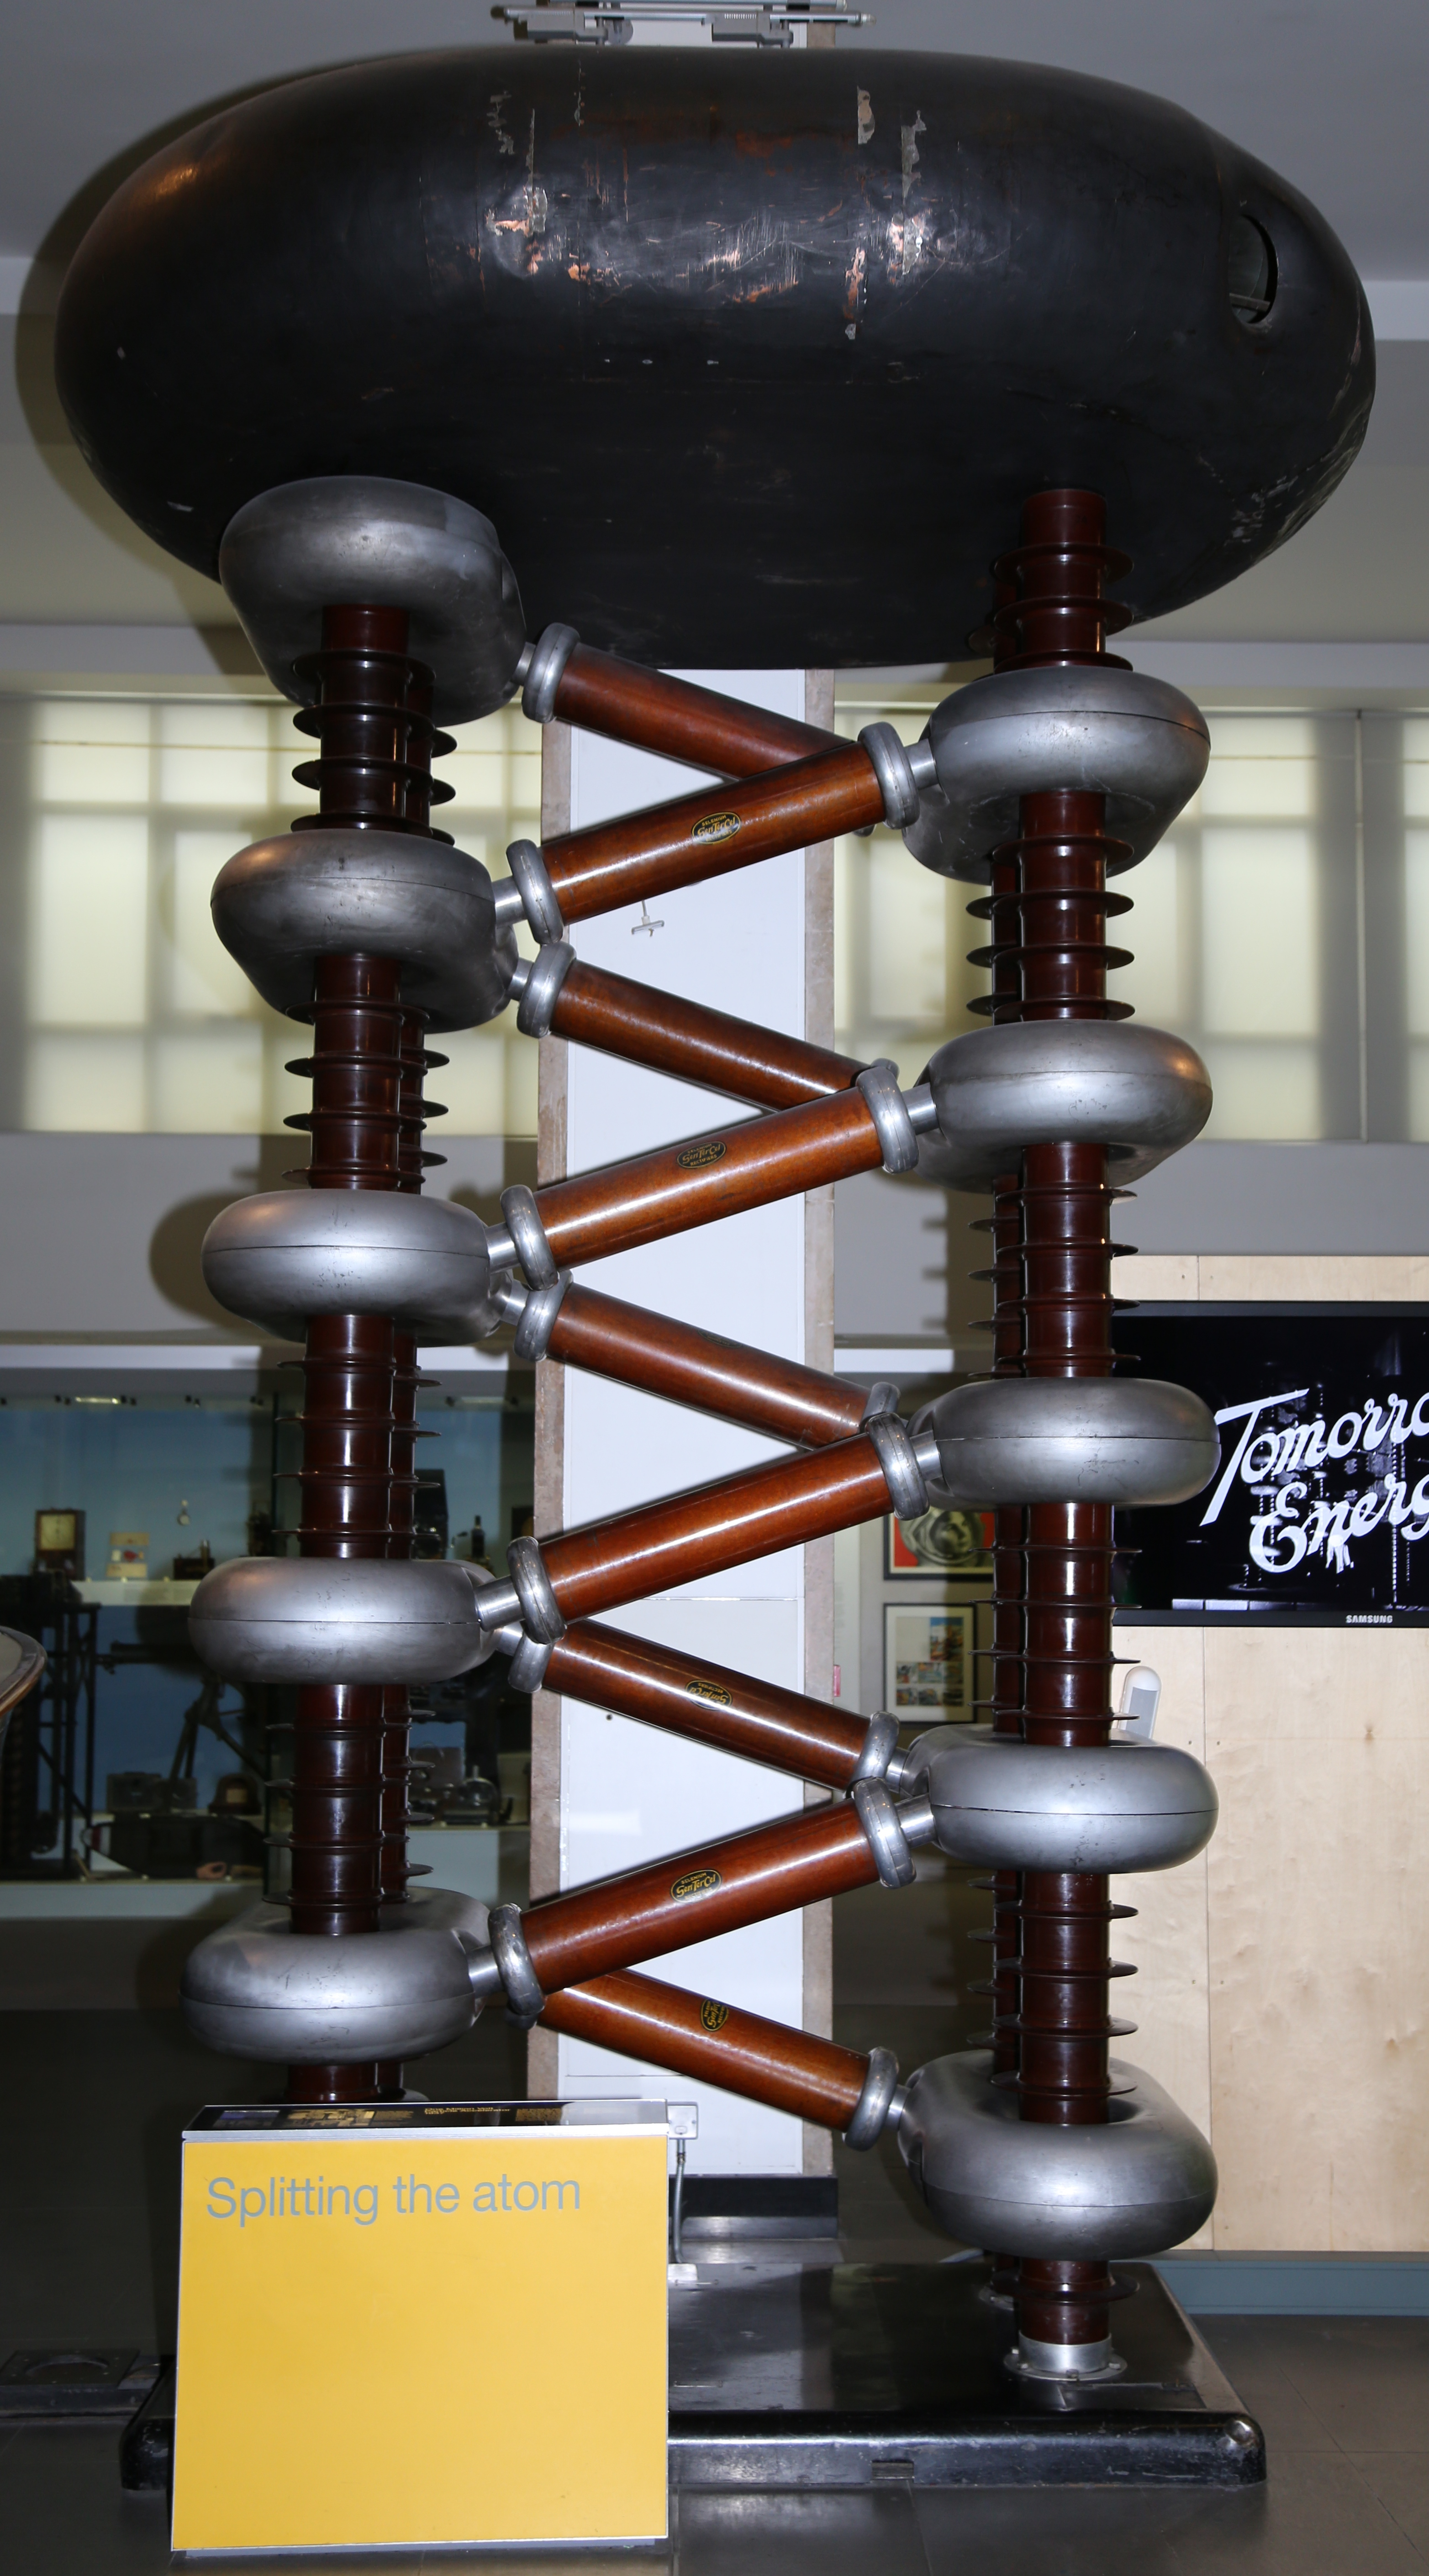
\includegraphics[width=6cm]{./1_modeling/img/CockcroftWaltonGenerator.jpg}
%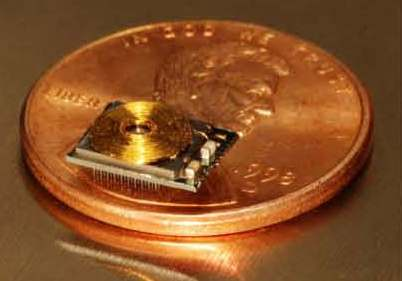
\includegraphics[width=6cm]{./0_intro/img/FSolzbacher01.jpg}
\caption{Cockcroft-Walton voltage multiplier built in 1937 by \emph{Philips Research Labs} in Eindhoven, now exposed in the \emph{Natural Science Museum} of London\\
\emph{Source:"Cockcroft–Walton generator 2012" by Geni. Licensed under GFDL via Wikimedia Commons  %http://commons.wikimedia.org/wiki/File:Cockcroft%E2%80%93Walton_generator_2012.JPG#/media/File:Cockcroft%E2%80%93Walton_generator_2012.JPG
}}
\label{fig:Cockcroft_VMR}
\end{figure}


In 1976, J.F. Dickson ~\cite{76Dickson} introduced a modification of the Cockcroft-Walton circuit to enable the integration of a voltage multiplier in an MNOS non volatile memory IC. The so-called Dickson charge-pump boosted the DC supply voltage proportionally to the number of stages in the pump. At same time, the new circuit mitigated the effects of the integrated capacitor stray capacitances on the voltage gain and reduced the output impedance of the converter increasing the current throughput. After the Dickson charge-pump other topologies~\cite{09Seeman} have been reported, such as the series-parallel converter ~\cite{94Ngo,94Cheong}, which allowed rational conversion ratios. F. Ueno \textit{et al.} ~\cite{91Ueno} presented yet another topology with conversion ratios corresponding to Fibonacci series,$k=1,2,3,5,8,..$ ,achieving higher conversion ratios using fewer capacitors ~\cite{95Makowski,09Allasasmeh}.  F.L. Luo  ~\cite{02Luo} proposed a topology cascading voltage doublers cells where the conversion ratio follows a quadratic relationship with the number of cells, and J. A. Starzyk ~\cite{01Starzyk} reviewed the same concept with a multi-phase topology that can achieve the same gain with fewer capacitors.



Two important concepts have been introduced to SC converters in order to reduce the current ripples and conduced Electromagnetic Interferences (EMI):
\begin{description}
  \item[Interleaving] also improves the efficiency since the it can reduce the value for the output capacitor. There are different reported implementations of 2-phase ~\cite{07Chang,99Chung}, 16-phase ~\cite{09Breussegem,14Andersen}, 32-phase~\cite{10Le} 64-phase~\cite{15Andersen}.
  \item[Current Mode] Charge-Pumps ~\cite{96Zhu,09Das} where the process of charge or discharge -or both- are controlled with a current source.
\end{description}

There are other innovative approaches where SCCs are combined with inductor based converters, also referred as \emph{hybrid} SCCs. The combination of both achieve large conversion ratios with tighter regulation. There are a large number of hybrid solutions where a SC cell is integrated into an inductor based converter ~\cite{05Axelrod,08Axelrod, 11Mayo,11Miranda,12Kline}. Lately, a couple of papers ~\cite{12Zhigang,11Dazhong} presented a Maximum Power Point Tracking (MPPT) converter for Photovoltaic (PV) cells employing a SC converter in parallel with an inductor based converter. This hybrid combinations offer another family of converters known as \emph{Resonant Switched Capacitor Converters} (RSCC), where the capacitors are charged through resonant transitions, thus eliminating the capacitor charge transfer losses.  K.W.E. Cheng ~\cite{01Cheng} in 2001 presented an early  work where in the topic using inductors limit the currents thought the capacitors and charging and discharging the capacitors with resonant transitions.  Subsequently, many publications appeared ~\cite{05Lee,10Cao,11Gebben,07Shoyama} presenting applications and uses of this converter family. Initial RSCC topologies made use of multiple inductors to guarantee a resonant transition for all capacitors, recent works~\cite{13Kesarwani,13Schaef,14Kesarwani,15Schaef} presented new topologies that reduced the number of inductors to achieve these resonant transitions.


\section{Sate of the Art of Switched Capacitor LED drivers}

One of the most popular application of SCCs is indeed as LED drivers for portable devices. Low power White LEDs (W-LEDs) are widely applied for back-lighting Liquid Crystal Display (LCD) in devices such as laptops, mobile phones and tablets. These applications require to generate a voltage above the LED forward voltage ($v_f$) from the battery, what can not been achieved with just using a linear drivers since the battery voltage is easily below to $v_f$  as it discharges. Normally theses drivers implement step-up or step-down to convert the battery right above the $v_f$.

\begin{figure}[t]
    \centering
    \begin{circuitikz} [scale=0.65]
    \ctikzset{bipoles/length=0.85cm}
   \draw[thick] (2.5,0.25) --
                (2.5,6.5) --
                (11.5,6.5) --
                (11.5,0.25) --
                (2.5,0.25);

    %Draw SCC block with capacitors
    \draw (3,1) --
          (3,6) --
          (5,6) --
          (5,1) --
          (3,1);

    \draw (4,1.25) node[rotate=90,anchor=west] {\emph{Multi-ratio SCC}};

    \draw (3,2) --
          (1.5,2) to[capacitor]
          (1.5,3) --
          (3,3);

    \draw (3,4) --
          (1.5,4) to[capacitor]
          (1.5,5) --
          (3,5);

    \draw (5,5.5) to[short,-o] (14,5.5);
    \draw (13,5.5) to[capacitor] (13,4.5) node[sground]{};

    \draw (4,1) -- (4,0) node[sground,scale=0.75]{};

   %Draw linear drivers
   \draw  (4,0.5) -- (10.5,0.5) -- (10.5,1);

   %First transitor
   \draw   (10,1) -- (10,1.5) node[npn,anchor=E,scale=0.5](npn1){}
           (npn1.C) -- (10,2.75) to[short,-o] (12,2.75);

   %Second transitor
   \draw  (10,1) -- (11,1)
           node[npn,anchor=E,scale=0.5](npn2){}
           (npn2.C) -- (11,2.25) to[short,-o] (12,2.25);

   %Controller box
   \draw (5.5,1) -- (8.5,1) -- (8.5,3) -- (5.5,3) -- (5.5,1);
   \draw (5.75,2) node[anchor=west, text width = 1.75cm]{Intensity Controller};
   \draw (npn2.B) -| (8.5,2);
   \draw (npn1.B) -| (8.5,2);

   %LEDs

   \draw [dashed] (14.25,5.5) to[short,o-] (15,5.5)
                    to[leD*] (15,2.75) to[short,-o] (12.25,2.75);

   \draw [dashed] (15,5.5) -- (17,5.5)
                    to[leD*] (17,2.25) to[short,-o] (12.25,2.25);

   %Add battery

   \draw (-1,0) node[sground,scale=0.75]{};
   \draw (-1,0) to[battery] (-1,6)
         -- (2.5,6);

    \end{circuitikz}
    \caption{Block diagram of a generic driver for backlighting applications.}
    \label{fig:backlight_LED}
\end{figure}

There is a large portfolio of available ICs, designated as Charge-Pumps (CPs), for driving LEDs in portable devices. Some commercial products are for instance  the \emph{MAX88779} \footnote{Maxim\textsuperscript{\textregistered} Charge Pump for Backlight/Flash/RGB LEDs with Safety Timer } or the \emph{MCP1252/3} \footnote{Microchip\textsuperscript{\textregistered} Low noise, Positive-Regulated Charge Pump}. These circuits  can drive withe, RGB or Flash LEDs from a Lithium-Ion battery only by adding a few external capacitors capacitors.  Generally these chips integrate an multi-target SCC with different conversion ratios (1:1, 3:2, 2:1) along with a series current regulator for each LED channel a shown in the block diagram of Figure~\ref{fig:backlight_LED}. Various publications ~\cite{07Feng,09Wu,10Yin} proposed enhancements in the architectures in order to reduce the parasitic losses bringing the efficiency close to the theoretical limit. Such drivers are used in applications below a 1$W$ and currents below hundred $mA$, their efficiency derates as the LED voltage moves away from the target voltage.

Besides the backlighting ICs, there are no other commercial LED drivers based on SCC. However that topic has been present in several research publications for the last years with few interesting publications targeting mains connected drivers. In 2008, K.H. Lee \emph{et al.}~\cite{08Lee} presented a SC step-down converter composed of several cascaded Series-Parallel that supplied from rectified 220$V_{rms}$ an LED string of 75V at 15W. In the proposed solution the LEDs are directly supplied using flying capacitors what produces pulsating currents in the string and its average values is controlled modulating the frequency of the converter. The cascaded topology minimized the number of components, switched and capacitors, for the required conversion ration (fixed by the LED string).

In 2012, M. Kline \emph{et al.} ~\cite{12Kline} proposed a isolated \emph{DC}/\emph{DC} converter that combined a SCC stage with series-LC resonant converter.  The SCC stage decreased  the rectified mains voltage, reducing the voltage stress in switches, capacitors and the elements of the resonant tank. The lower voltage stress allows a reduction in the volume of the passive components and the total area in the silicone. By controlling the frequency and the duty cycle of the SCC stage current through the LEDs can be regulated, resulting in a very efficient solution. In a recent publication they presented an implementation where power train and control where integrated in different stackable ICs modules~\cite{13Kline}.

The different applications show an increasing interest in using SCC for LED drivers. It is evident that the approach used in portable devices can no be further extended in for high powers and higher voltages. The use of a bear SCC can never satisfy the requirements of LED drivers due to the following facts:
\begin{itemize}
  \item Only provide voltage-to-voltage conversion
  \item Fixed conversion ratios
  \item Regulation is provided by series shunting
\end{itemize}
These limitations combined with the abrupt characteristics I-V of the LEDs makes barely impossible to provide high efficient solutions with the single use of SCC. The converters would require to have a large number of conversion ratios with a very large granularity to avoid uncontrolled currents flowing through the LEDs.

The research presented in this work aims to explore the possibilities of the SCC for LED drivers and the conducting path is based in the combination of the with inductors. The overall solution improves the power density and reduced form factor of the present solutions.



\section*{Power Levels and Integration}

There are not intrinsic implications that limit the output power of a Switched Capacitor converter, but the boundary conditions. There are implementations ranging from tens of milliwatts to tens of kilowatts, where the difference only relies in the used technology. They can be classified in 3 groups: Fully integrated circuits, integrated circuits with external capacitors and discrete solutions.

Full integrated converter are suitable for very lower power applications from some microwatts up to some tens of milliwatts. These solutions are implemented in standard processes (CMOS, BiCMOS or Bipolar) where the priority is in achieve an integrated solution rather than efficient. These converters have very poor efficiency up to 60\%, due to the low energy density and poor quality of the capacitors available in those processes. The second group overcomes this problem using external capacitors. These converters integrate the control and the power train in a single chip with a stadard CMOS process, offering  output power up to one watt and peak efficiencies of 95\%. In this case, the CMOS switches limit the converter efficiency and scalavility in power.
The implementations with discrete components enable output powers up to kilowatts with peak efficiencies above 95\%. Discrete semiconductor switches can offer lower channel resitance and better switching characterisitcs, reducing ohmic resitance and enabeling higher switching frequencies.  \emph{ \color{red} Silicon power MOSFET are the dominant in discrete implementations, but recent publications used Galiun-Nitride HEMT switches ~\cite{11Scott,12Scott}}.

The limiting factor of the output power of a SC converter is driven by the boundary conditions of the technology. Up to now, integrated SC converters designs have been covered addressing the problem with the standard process in VLSI, in order to have compact power conversion units at the lowest cost. The current technologies can easily improve the present solutions, for instance, a Power-System on Package (PSoC) integrating switches and capacitors would already reduce the series resistance of the pins and optimize the silicon die area of the present integrated converters with external capacitors. The current technologies offer the possibility to achieve integrated SC converters processing higher powers, but it would require to combine them in non-standard processes.

\emph{\color{red} Missing refs!}


%\bibliographystyle{plainnat}
%\bibliography{phd_bib} 


\chapter[Advanced Modeling of SCC]{Advanced Modeling of Switched Capacitor Converters}

\section{Introduction}

\section{Single Output Converters}
Switched Capacitor Converters (SCCs) are considered to be a two-port converter with single input and a single output as shown in Fig.\ref{fig:two_port}. The input port is connected to a voltage source and the output port feeds the load. The SCC provides between input, $v_i$, and output, $v_o$, a voltage conversion, $m$,  that  steps up, steps down or/and inverts the polarity of the input voltage. Up to present all the circuit theory devoted SCCs is valid only for the two-port configuration, therefore this section is dedicated to revisit the classical concepts of single output SCC and to introduce new ones that enable a broader use of such converters.

\begin{figure}[!h]
\centering
\ctikzset { bipoles/length=1cm}
\begin{circuitikz}[scale=0.65]
\draw
    (1,0) to[short,o-]
    (0,0) to[V = $V_{supply}$]
    (0,3) to[short,-o]
    (1,3) ;

\draw
    (2,3) --
    (2.5,3)

    (2,0) --
    (2.5,0)

    node[ocirc]  (IC)  at (2,0) {}
    node[ocirc]  (I) at (2,3) {}
    (I) to[open,v=$v_{i}$] (IC);


\draw [thick]
    (2.5,-0.5) --
    (2.5,3.5)  --
    (5.5,3.5)  --
    (5.5,-0.5) --
    (2.5,-0.5);

\draw (4,2)node[anchor=north]{$\frac{v_o}{v_{i}}=m$} ;
\draw
    (5.5,3) -- (6,3)
    (5.5,0) -- (6,0)
    node[ocirc]  (O)  at (6,3) {}
    node[ocirc]  (OC) at (6,0) {}
    (O) to[open,v^<=$v_{o}$] (OC);

\draw
    (7,0) to[short,o-]
    (8,0) to[ R= $Load$,mirror]
    (8,3) to[short,-o]
    (7,3) ;
\end{circuitikz}
\label{fig:two_port}
\caption{General two port configuration of a Switched Capacitor Converter. }
\end{figure}


\subsection[Introducing H-SCC]{The Hybrid-SCC: Identifying Outputs in Switched Capacitor Converters}

Two types of nodes can be identified in a Switched Capacitor Converter, as shown in Fig. \ref{fig:dc_pwm_nodes}:
\begin{itemize}
  \item Fixed voltage \emph{dc}-nodes, node $a$ % node $a$ in Fig. \ref{fig:dc_pwm_nodes}
  \item Floating voltage \emph{pulsed width modulated}-nodes (\emph{pwm}-nodes),  node $b$ % in Fig. \ref{fig:dc_pwm_nodes}
\end{itemize}



\begin{figure}[!h]
\centering
\ctikzset { bipoles/length=1cm}
\begin{circuitikz}[american voltages,scale=0.65]
\draw
        %Draw Switches
        (0,0)  to[V=$V_{in}$]
        (0,8)  --
        (5,8)   to[switch=$\phi_1$]
        (5,6)   to[switch=$\phi_2$]
        (5,4)   to[switch=$\phi_1$]
        (5,2)   to[switch=$\phi_2$]
        (5,0)  --
        (0,0)

        (5,6) to[short,-o]
        (8,6) node[anchor=west] {$b \rightarrow$  \emph{pwm}  node}

        (5,4) to[short,-o]
        (8,4) node[anchor=west] {$a \rightarrow$ \emph{dc} node}

%Draw Capacitors
        (5,2) --
        (3,2) to[C=$C_{fly}$]
        (3,6)--
        (5,6)

        (5,0) --
        (7,0) to[C=$C_{dc}$,mirror]
        (7,4)--
        (5,4);
 \draw (5,7) node[anchor=east]{$S_1$}
       (5,5) node[anchor=east]{$S_2$}
       (5,3) node[anchor=east]{$S_3$}
       (5,1) node[anchor=east]{$S_4$} ;

  \begin{scope}[xshift=13cm,yshift=0.2cm]
  \draw [->] (-0.1,0) -- (5,0) node[anchor=west]{$t$};
  \draw [->] (0,-0.1) -- (0,2.5) node[anchor=east]{$v_a$};
  %\draw (0,-1) node[anchor=south]{0}
%        (1.25,-1) node[anchor=south] {$T$}
%        (2.5,-1)  node[anchor=south] {$2T$}
%        (3.75,-1) node[anchor=south] {$3T$} ;

  \draw [thick] (0,1) -- (0.75,0.75) -- (0.75,0.95) -- (1.25,0.80)
                      -- (1.25,1)-- (2,0.75) -- (2,0.95) -- (2.5,0.80)
                      -- (2.5,1)-- (3.25,0.75) -- (3.25,0.95) -- (3.75,0.80);

  \draw [dashed] (0,0.875) -- (4,0.875) node[anchor=west]{$v_a$} ;
  \end{scope}

  \begin{scope}[xshift=13cm,yshift=4 cm]
  \draw [->] (-0.1,0) -- (5,0) node[anchor=west]{$t$};
  \draw [->] (0,-0.1) -- (0,2.5) node[anchor=east]{$v_b$};
  %\draw (0,-1) node[anchor=south]{0}
%        (1.25,-1) node[anchor=south] {$T$}
%        (2.5,-1)  node[anchor=south] {$2T$}
%        (3.75,-1) node[anchor=south] {$3T$} ;

  \draw [thick] (0,2) -- (0.75,1.85) -- (0.75,1) -- (1.25,0.80) --
                (1.25,2) -- (2,1.85) -- (2,1) -- (2.5,0.80) --
                (2.5,2)-- (3.25,1.85) -- (3.25,1) -- (3.75,0.80);

  \draw [dashed] (0,1.515) -- (4,1.515) node[anchor=west]{$v_b$} ;
  \end{scope}

\end{circuitikz}
\caption {Nodes types in a SCC. Node $a$ is a \emph{dc}-node; its voltage, $v_a$ is plotted in the bottom graph. Node $b$ is a \emph{pwm}-node; its voltage, $v_b$, is plotted in the top graph.   }
\label{fig:dc_pwm_nodes}
\end{figure}

 The fixed voltage \emph{dc}-nodes are the common used nodes to supply a \emph{dc} load. They provide a fixed voltage conversion defined by the topology with a low \emph{ac} ripple, and they always have connected a capacitor between the node and the ground by the so called \emph{dc}-capacitor as shown in the Fig. \ref{fig:dc_pwm_nodes}. Depending on the topology the number of \emph{dc}-nodes can vary between one or more, however topologies that reduce the number of \emph{dc}-capacitors ($C_{dc}$) trend to have a better utilization of the capacitors since \emph{dc}-capacitors do not contribute to transport charge \cite{09Seeman}.\\


 The floating \emph{Pulsed Width Modulated}-nodes (\emph{pwm}-nodes) have been rarely used as outputs until a recently  couple of publications \cite{12Kumar,12Kline} presented the advantages of using them. \emph{pwm}-nodes have been normally considered just internal to the converter with any added value, but actually the conversion possibilities of SCCs can be further exploited by using these nodes as outputs.


A \emph{pwm}-node is located a the terminal of a \emph{flying capacitor} ($C_{fly}$) and provides a floating \emph{Pulsed-Width-Modulate} voltage with an added \emph{dc} offset of a fraction of the input voltage. The magnitudes are related to the SCC topology. The pulsated voltages can be filtered using an inductive-capacitive filter (\emph{LC}) allowing to supply \emph{dc} load with averaged voltage of the node. Actually the \emph{pwm} voltage at the node can be controlled adjusting the duty
cycle of the SCC, enhancing the regulation capabilities of these outputs compared to the fixed value of the \emph{dc}-nodes.
The switched capacitor converters that combine the \emph{pwm}-outputs with inductors will be referred from now on as
\emph{Hybrid}-Switched Capacitor Converters (H-SCC).




\subsection{The Output Impedance Model}


\begin{figure}[!h]
\centering
\ctikzset { bipoles/length=1cm}
\begin{circuitikz}[scale=0.65]
\draw
    (5,0) to[short,o-]
    (0,0) to[V = $V_{target}$]
    (0,3) to[R=$R_{scc}$,-o]
    (5,3)

    (5,0) to[open,v_>=$v_o$] (5,3);


\end{circuitikz}
\label{fig:OI_model}
\caption{The Output Impedance Model for SCCs. }
\end{figure}

\begin{figure}[!h]
\centering
%\input{./1_modeling/imgs/test_plot.tex}
\label{fig:SINE}
\caption{The Output Impedance Model for SCCs. }
\end{figure}






\subsection{Identifying the source of losses in the charge transfer}
\subsection{Re-formulating the charge flow analysis}
\subsubsection[SSL Capacitor Charge Flow]{Slow Switching Limit: Re-defining the Capacitor Charge Flow Vectors}
\subsubsection[FSL Switch Charge Flow]{Fast Switching Limit: Re-defining the Switch Charge Flow Vectors}

\subsection{Load Model: Voltage Sink versus Current Sink}
\subsection{Sensitivity of the inductor current ripple}

\section{Multiple Output Converters}
\subsection{The Output Trans-Resistance Model}
\subsection{Obtaining the Trans-Resistance parameters with the charge flow analysis }













\chapter[Optimization and Design]{Optimization and Design of Hybrid-Switched Capacitor Converters}
\section{Introduction}
\section{Study in the correlation of the design parameters and the Output Impedance}
\section{Encapsulating the Switches and Capacitors area breakdown in an optimization procedure}
\section{Insights towards a complete optimization}

\chapter[Dynamic Study]{Dynamic Study of Hybrid-Switched Capacitor Converters}
\section{Small Signal Analysis}


\part{Hybrid Switched Capacitor Converter based architectures for LED Drivers }

\chapter{An experimental setup for validating the proposed model}
\section{Circuit description}
\section{Identifying the losses}
\subsection{Switching Losses}
\subsection{Characterization the switches $R_{ON}$ }
\subsection{Fast Switching Limit Losses}
\subsection{Slow Switching Limit Losses}
\section{Playing with the design space}
\subsection{Validating the SSL optimization}
\subsection{Validating the FSL optimization}

\section{Results}
\section{Conclusions}
\chapter{12W H-SCC LED Architecture}
\section{Introduction}
\section{Circuit Description}
\section{Design and Implementation}
\section{Results}



\chapter{AC/DC Architecture}
\section{Introduction}
\section{Circuit Description}
\section{Design and Implementation}
\section{Results}
\subsection{Model verification}
\part{Guidelines towards integration}
\section*{Introduction}

\chapter{Mega-LED platform}


%\bibliographystyle{plain}
\bibliographystyle{plainnat}
\bibliography{phd_bib}

\end{document}


